Selecting the switching circuitry consists of four different parts, the switches, drivers, optocouplers and the heat sink. Additional support circuitry will be designed, when selecting the commercial components.

\subsubsection{Switch sizing} \label{switch_sizing}
The system must regulate the power flow in order to maximize the power generation. In order to achieve this, the system includes switches that control the current flow. The switches consist on MOSFET devices. The switching frequency of the system is selected to be $50kHz$. Although the market has IGBT which can switch at $50kHz$, MOSFET devices allow lower losses than IGBTs for system's current rating \cite{mosfet_igbt_switching_loss} \cite{igbt_or_mosfet}.


The maximum output voltage of the system is $90V$, however the voltage rating of the transistors was set to $150V$ in order to consider a safety margin, and thus, increase the reliability. The peak current through the transistors happens when the buck mode is active and the maximum number of MICs are used in series. The peak current is equal to $14A$. In order to reduce the conduction losses and the heat sink size, a low on resistance is desired shown in equation \ref{conduction_losses_eq}\cite{mosfet_losses}. These constraints were used when searching for the ideal component. The chosen device is the IPB200N15N3. It exhibits the features seen in table \ref{mosfet_features}.


\begin{table}[htbp]
	\centering
	\begin{tabular}{|p{6cm}|>{\centering}p{6cm}|}
		\hline
		\rowcolor{lightgray}\multicolumn{2}{|l|}{ \textbf{Maximum ratings}} \\ \hline
		Continuous $I_{D}$ & 40 [A]  \tabularnewline \hline
		$V_{GS}$ & $\pm$ 20 [V]  \tabularnewline \hline
		Power dissipation & 150 [W]  \tabularnewline \hline
		$V_{DS}$ & 150 [V]  \tabularnewline \hline
		$R_{DSon} $ & 20 [m$\Omega$]  \tabularnewline \hline
		\rowcolor{lightgray}\multicolumn{2}{|l|}{ \textbf{Other values of interest}} \\ \hline
		Input capacitance & 1820 [pF]  \tabularnewline \hline
		Package & D2PAK  \tabularnewline \hline
		$V_{th} $ $(V_{GS} = 3 V)$ & 3 [V]  \tabularnewline \hline
		$V_{th} $ $(V_{GS} = 36 V)$ & 4.7 [V]  \tabularnewline \hline
		$R_{Gate} $ & 2.4 [$\Omega$]  \tabularnewline \hline
	
	\end{tabular}
	\caption{MOSFET figures of merit. T = 25 $\decC$ \cite{mosfet_datasheet}.}
	\label{mosfet_features}
\end{table}

\subsubsection{Heat sink sizing}

The procedure followed for validating the heat sink might be seen at figure \ref{heat_sink_validation_procedure}. If the total temperature increase is within switch's safe operating area, then the heat sink is providing enough heat dissipation.

\begin{figure}[htbp]
	\begin{center}
		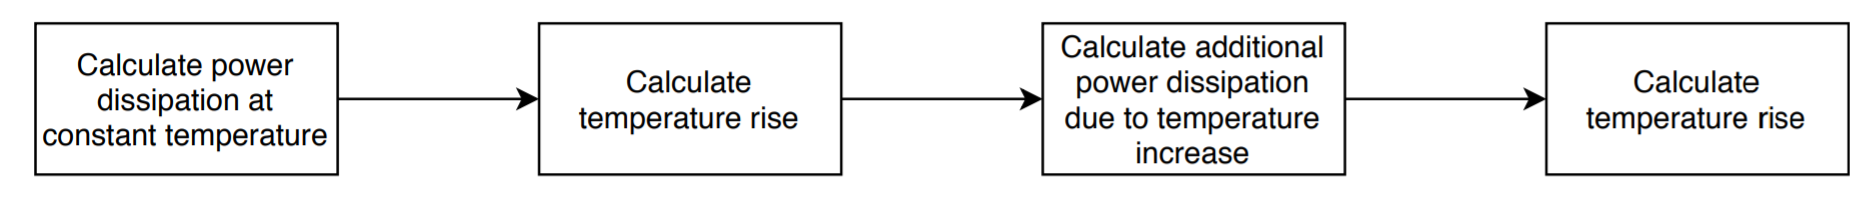
\includegraphics[width=\textwidth]{../Pictures/P1/Component_sizing/heat_sink_validation_procedure.png}
		\caption{Heat sink validation procedure.}
		\label{heat_sink_validation_procedure}
	\end{center}	
\end{figure}

The power dissipated in the switches is equal to the sum of the conduction losses and the switching losses. The conduction losses might be calculated  as seen in equation \ref{conduction_losses_eq}.

\begin{equation} \label{conduction_losses_eq}
P_{cond} = i(t)^2 \cdot R_{DS}
\end{equation}

The switching losses depend upon the switching frequency and the transistor's manufacturing characteristics\cite{mosfet_losses}. In order to calculate the value, the MOSFET's SPICE model was obtained from the manufacturer's website. The next step was to perform the simulation of the system. The system was simulated in both buck and boost modes. Special attention was put into the dead-band between PWM signals of different switches, to avoid current shoot through. After simulating, the average power dissipation under steady state was calculated in both modes. Within every mode, the simulation was performed under the most unfavorable conditions, this is: buck's output is 24 V and boost's output is 90 V. The results can be seen in table \ref{mosfet_final_dissipation}, column 1.

The datasheet shows that the $R_{DS}$ variation is mainly dependent on the temperature\cite{mosfet_datasheet}. The models found neglect the temperature difference. Then, in order to get an approximated value considering temperature, the procedure will be to calculate the total losses at constant temperature using the SPICE model and then add the additional conduction losses due to the increase of the resistance, as expressed by equation \ref{total_losses}.


\todo{Since you have made the simulations it would be a good idea to add them as appendices and refer to them. AT. Might be a good idea. Lets see if the limits of the document allows us (maximum number of pages).}

\begin{equation} \label{total_losses}
\overline{P} = \overline{P_{loss, T = K}} + \overline{i(t)^2 \cdot \Updelta R_{DS}}
\end{equation}

Now the junction temperature based on the power dissipation, calculated using the SPICE model, is calculated. The ambient temperature is set to 50 $\decC$, which is considered a realistic scenario \todo{ref}. The thermal circuit can be seen in figure \ref{thermal_circuit}. The next step is to choose a commercial heat sink. The constraints are thermal resistance, size and price. TDEX6015/TH was found. Its features might be found in table \ref{heatsink_features}. The switches temperature will be analysed in order to validate the heat sink. The analysis considers all the transistors as a single power source.

\begin{figure}[H]
	\begin{center}
		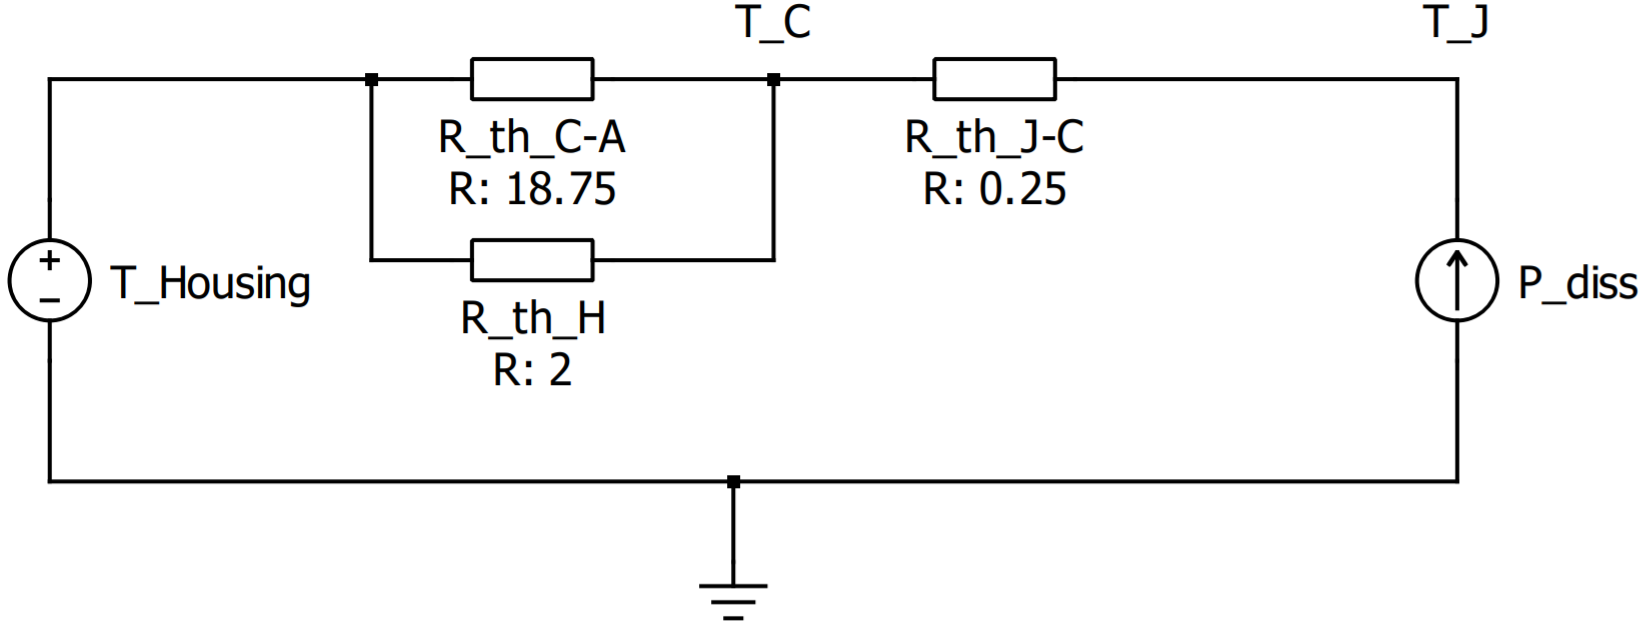
\includegraphics[width=0.7\textwidth]{../Pictures/thermal_circuit.png}
		\caption{Thermal circuit used for sizing the heat sink}
		\label{thermal_circuit}
	\end{center}	
\end{figure}

\begin{equation} \label{switch_temperature}
T_{J} = T_{housing} + \overline{P_{loss, T = K}} \cdot  R_{thermal}
\end{equation}


If no heat sink were used, according to equation \ref{switch_temperature}, the junction temperature would become too high and the components would be damaged. See equation \ref{temperature_without_heatsink}. This is mainly explained due to the fact that the thermal resistance between junction and ambient of the transistor is as high as 75 $\decC / W$.

\begin{equation} \label{temperature_without_heatsink}
T_{J} = 50 \decC + 5.54 W \cdot 75 \frac{\decC}{W} = 465.5 \decC
\end{equation}


\begin{table}[htbp]
	\centering
	\begin{tabular}{|p{6cm}|>{\centering}p{8cm}|}
		\hline
		\rowcolor{lightgray}\multicolumn{2}{|l|}{ \textbf{Features}} \\ \hline
		Size & 60x60x16 [mm]  \tabularnewline \hline
		Thermal resistance & 2.06 [K/W]  \tabularnewline \hline
		
	\end{tabular}
	\caption{Heat sink figures of merit \cite{heatsink_datasheet}.}
	\label{heatsink_features}
\end{table}


\begin{equation} \label{switch_temperature_w_values}
T_{J} = 50 \decC + 5.54 W \cdot  2.06\frac{\decC}{W} = 61.41 \decC
\end{equation}

The drain-to-source resistance increase is calculated as explained in equation \ref{delta_resistance}. The resistance difference is relatively small. The resistor at every temperature was collected from the component data sheet.

\begin{equation} \label{delta_resistance}
\Updelta R_{DS} = |R_{DS, T = 20 \decC} - R_{DS, T = 61.41\decC}| = 4\; m \Omega
\end{equation}

\begin{table}[]
	\centering
	\begin{tabular}{|l|l|l|l|}
		\hline
		\rowcolor[HTML]{C0C0C0} 
		\multicolumn{4}{|c|}{\cellcolor[HTML]{C0C0C0}\textbf{Switches power dissipation}}                                                   \\ \hline
		\rowcolor[HTML]{C0C0C0} 
		Switch         & $\overline{P_{loss, T = K}}$ {[}W{]} & $ \overline{i(t)^2 \cdot \Updelta R_{DS}}$ {[}W{]} & \textbf{Total {[}W{]}} \\ \hline
		\multicolumn{4}{|l|}{Buck mode}                                                                                                     \\ \hline
		M1             & 2.91                                 & 0.39                                               & \textbf{3.30}          \\ \hline
		M2             & 0.82                                 & 0.21                                               & \textbf{1.03}          \\ \hline
		M3             & 1.81                                 & 0.58                                               & \textbf{2.39}          \\ \hline
		M4             & 0                                    & 0                                                  & \textbf{0}             \\ \hline
		\textbf{Total} & 5.54                                 & 1.18                                               & \textbf{6.72}          \\ \hline
		\multicolumn{4}{|l|}{Boost mode}                                                                                                    \\ \hline
		M1             & 0.69                                 & 0.28                                               & \textbf{0.97}          \\ \hline
		M2             & 0                                    & 0                                                  & \textbf{0}             \\ \hline
		M3             & 0.48                                 & 0.12                                               & \textbf{0.6}           \\ \hline
		M4             & 3.31                                 & 0.18                                               & \textbf{3.49}          \\ \hline
		\textbf{Total} & 4.48                                 & 0.58                                               & \textbf{5.06}          \\ \hline
	\end{tabular}
\caption{Power dissipation analysis. Column 1, average power dissipation at constant 25 $\decC$ temperature. Column 2, extra power dissipation due to the increase of temperature.}
\label{mosfet_final_dissipation}
\end{table}


The full power dissipation values can be found on table \ref{mosfet_final_dissipation}. To achieve an exact result, an iterative process should be followed. However, after the first iteration, the change ratio is extremely small and then, neglected. Now that the power dissipation has been calculated, the junction temperature must be checked in order to confirm that the heat sink has been properly sized. Equation \ref{switch_temperature} is used, substitution of values leads to \ref{switch_temperature_w_values_2}. The difference is fairly small and the junction temperature remains within safe area. Then, TDEX6015/TH has been validated as a proper heat sink.

\begin{equation} \label{switch_temperature_w_values_2}
T_{J} = 50 \decC + 6.72 W \cdot  2.06 \frac{\decC}{W} = 63.84 \decC
\end{equation}